\documentclass[11pt,a4paper]{article}

\usepackage[utf8]{inputenc}
\usepackage[T1]{fontenc}
\usepackage{lmodern}
\usepackage[margin=1in]{geometry}
\usepackage{amsmath, amssymb, amsthm}
\usepackage{graphicx}
\usepackage{booktabs}
\usepackage{caption}
\usepackage{subcaption}
\usepackage{hyperref}
\usepackage{xcolor}
\hypersetup{colorlinks=true, linkcolor=black, citecolor=blue, urlcolor=blue}
\usepackage{enumitem}
\usepackage{microtype}
\usepackage{authblk}
\usepackage{float}
\usepackage[round,authoryear]{natbib}
\bibliographystyle{plainnat}

\title{\Large{\bf Network-Augmented Latent Factor Portfolios for Cryptocurrencies}\\[3pt]
\large{A Crypto Factor Zoo with Giglio--Xiu Hidden-Factor Pricing}}

\author{Artemis Quant Competition Submission --- 2026 cycle}
\affil{Track 1: Crypto Factor Rebalancing Strategy}
\date{\today}

\begin{document}
\maketitle

\begin{abstract}
\noindent We build a \emph{Crypto Factor Zoo} of nine economically-motivated long/short factor portfolios drawn from three established research lines --- the Fama--French-analogue factors of \citet{hartmann2025hidden}, the community-based momentum signals of \citet{liu2018timevarying}, the supply / cash-flow factors of the parent project's RAAM~v2 stage, and the betting-against-beta low-volatility anomaly of \citet{frazzinipedersen2014} --- and price them jointly with hidden risk factors using the three-pass framework of \citet{giglioxiu2021}. The number of hidden factors is selected by Bai--Ng (2002) IC$_{p2}$. On 52 weekly observations of an 85-asset crypto universe (2025-05-12 to 2026-05-04) we find that \textbf{five of seven observed factors clear the $|t|\!\ge\!1.65$ significance bar} in the cross-sectional Fama--MacBeth regression: low-volatility ($t=+4.27$), momentum ($+3.44$), within-cluster momentum ($+3.37$), cross-cluster relative strength ($+3.37$) and size ($+3.00$). When the model is converted into a weekly long/short quintile portfolio with cluster, asset, turnover and volatility constraints, the in-sample Sharpe is 2.30 but the out-of-sample Sharpe over 24 weeks is $-1.44$ with a 95\% block-bootstrap CI of $[-3.45,\, 1.18]$ that straddles zero. The cross-section of factor premia is statistically real; the *headline* L/S quintile combination does not generalise reliably in this sample. We report the result honestly and discuss what would have to be different for the strategy to be vault-deployable.
\end{abstract}

\vspace{0.5em}
\noindent\textbf{Track.} 1 --- Crypto Factor Rebalancing Strategy.\\
\noindent\textbf{Code.} \texttt{08\_nalfp/} on the project repository; full pipeline runs end-to-end in under three minutes.

\section{Introduction}

The Artemis competition rubric weights ``Signal / Edge Validity'' (30\%) and ``Critical Evaluation'' (20\%) at half the total score and explicitly favours methodological honesty over backtested glamour \citep{artemis2026competition}. We take both clauses seriously. This paper is structured around a single empirical question:

\begin{quote}
\emph{Which crypto-native risk factors carry a statistically priced risk premium in our sample, and does that pricing translate into out-of-sample tradability after honest costs and constraints?}
\end{quote}

The answer turns out to be: \emph{five factors are priced in-sample with $t$-stats above 3, but a long/short quintile portfolio built on the implied expected-return rank does not generalise on the 24 out-of-sample weeks we have to test it on.} We treat this as a clean negative-result-with-strong-mechanics finding and report it transparently.

\paragraph{Three contributions.}
\begin{enumerate}[topsep=2pt,itemsep=0pt]
\item A \emph{Crypto Factor Zoo} of nine long/short factor portfolios, each sourced from a specific paper with explicit construction recipes and economic narratives (Section~\ref{sec:zoo}).
\item A \citet{giglioxiu2021} three-pass implementation that prices the zoo jointly with hidden factors selected by Bai--Ng IC$_{p2}$ (Section~\ref{sec:gx}).
\item A weekly long/short portfolio overlay built on top of the GX expected return, plus a transparent out-of-sample backtest with stationary block-bootstrap Sharpe CIs (Sections~\ref{sec:portfolio}--\ref{sec:critique}).
\end{enumerate}

\section{Data and universe}\label{sec:data}

The universe is the 85 non-stablecoin, non-wrapped, non-bridged cryptocurrencies for which complete weekly market and Artemis fundamentals exist over 2025-05-12 to 2026-05-04 (52 weeks). Prices come from CoinGecko daily ticks aggregated to Monday close. Stablecoins, wrapped tokens (e.g.\ WBTC) and bridged tokens are excluded up front. Every weekly characteristic --- momentum, volatility, log market cap, dollar-volume turnover, TVL/mcap, fundamental yield, supply absorption, activity growth --- is lagged by one period so the panel admits no look-ahead.

\section{The Crypto Factor Zoo}\label{sec:zoo}

Factor portfolios are formed weekly by sorting the cross-section on a single characteristic, going long the top tercile and short the bottom tercile (equal-weighted within each leg), except where noted.

\subsection{Construction and economic story}

\begin{description}[topsep=2pt,itemsep=2pt,leftmargin=1.2em]
\item[RC --- crypto market.] Value-weighted return of the universe using lagged market caps. The \citet{hartmann2025hidden} RC factor; CAPM-analogue broad-market premium. Expected sign is regime-dependent.
\item[SMBC --- size.] Long bottom 30\% by lagged $\log$\,mcap, short top 30\%. The Fama--French SMB analogue for crypto \citep{hartmann2025hidden, famafrench1993}. Small-cap names historically have higher returns at higher fundamental and liquidity risk. Expected sign $+$ in risk-on regimes.
\item[MomC --- momentum.] Long top 30\% by trailing 4-week return, short bottom 30\%. The strongest documented cross-sectional anomaly in crypto \citep{liu2022commonrisk, jegadeeshtitman1993, carhart1997}. Expected sign $+$.
\item[VolC --- low-volatility.] Long bottom 30\% by 4-week realised vol, short top 30\%. The betting-against-beta anomaly \citep{frazzinipedersen2014}: leverage-constrained investors over-bid high-vol names. Expected sign $+$ (low-vol premium positive).
\item[TVLC --- DeFi engagement.] Long top 30\% by TVL/mcap, short bottom 30\%. The argument is that protocols with high TVL/mcap have market values anchored by genuine on-chain usage \citep{hartmann2025hidden}; the \citet{yousaf2025tvlirrelevance} paper finds $\alpha\!\approx\!0$ after market/size/momentum controls. We include TVLC explicitly to test that finding in our sample.
\item[FunC --- fundamental yield.] Long top 30\% by $F=(\text{fees}+0.5\cdot\text{rev})/\text{mcap}$, short bottom 30\%. The crypto ``value'' factor: cash flow per dollar of market cap. Source: RAAM v2 stage 04 of this project. Coverage is sparse (62\% missing); most assets do not produce fee revenue.
\item[SupC --- supply absorption.] Long top 30\% by supply-absorption rank (low emission), short bottom 30\%. Tokens with low net new supply face less structural sell pressure from emissions \citep{raamv2}. Coverage in our 52-week sample is severe (85\% missing) so we report the factor stat but exclude it from GX.
\item[NetMom --- within-cluster momentum.] \emph{Within each Louvain cluster} (Section~\ref{sec:pillar1}), long top half by within-cluster momentum rank, short bottom half; average across clusters. Cluster-neutral by construction. Implements \citet{liu2018timevarying} §4 ``community-based momentum''.
\item[NetRel --- cross-cluster relative.] Long top 30\% by own 4-week return minus the mean 4-week return of \emph{other} clusters, short bottom 30\%. Captures narrative rotation \emph{across} communities, distinct from MomC because it normalises against cross-cluster averages.
\end{description}

\subsection{Full-sample factor statistics}

\begin{table}[H]
\centering
\caption{Factor Zoo --- full-sample weekly statistics. ``IC'' is the time-series-averaged Spearman correlation of the sorting characteristic with the next-week return.}
\label{tab:zoo}
\small
\begin{tabular}{lrrrrrrr}
\toprule
Factor & $n$ & Ann.Mean & Ann.Vol & Sharpe & NW $t$ & MaxDD & IC \\
\midrule
RC      & 50 & $-32.4\%$ & $41.8\%$ & $-0.78$ & $-0.74$ & $-51.6\%$ & --- \\
SMBC    & 51 & $+93.7\%$ & $26.5\%$ & $+3.54$ & $+2.90$ & $-14.9\%$ & $+0.015$ \\
MomC    & 48 & $+40.0\%$ & $36.7\%$ & $+1.09$ & $+1.16$ & $-24.5\%$ & $+0.026$ \\
VolC    & 49 & $+10.0\%$ & $46.2\%$ & $+0.22$ & $+0.22$ & $-31.3\%$ & $+0.090$ \\
FunC    & 50 & $+26.6\%$ & $31.4\%$ & $+0.85$ & $+1.05$ & $-18.4\%$ & $+0.001$ \\
SupC    & 7  & $+51.8\%$ & $17.7\%$ & $+2.93$ & --- & $-1.8\%$ & $+0.098$ \\
NetMom  & 40 & $+30.4\%$ & $22.9\%$ & $+1.33$ & $+1.19$ & $-19.6\%$ & $+0.006$ \\
NetRel  & 40 & $+74.8\%$ & $33.4\%$ & $+2.24$ & $+2.14$ & $-18.6\%$ & $+0.046$ \\
\bottomrule
\end{tabular}
\end{table}

\noindent\textbf{Three takeaways.}
(i) \emph{SMBC and NetRel are the two strongest factors in this sample} with Newey--West $t$-stats above 2. Small caps dominated and cross-cluster narrative rotation was a strong predictor.
(ii) \emph{The market factor RC is negative} (Sharpe $-0.78$): the universe was net-down over 52 weeks. This contextualises the long/short factor performance --- the strong SMBC return is partly a flight from majors into a few outperforming small-caps.
(iii) \emph{TVLC has zero usable observations}: $\text{tvl\_to\_mcap}$ is missing for nearly the entire universe because most assets don't have a measurable DeFi TVL. SupC has only seven observations. Both factors are excluded from the GX panel.

\begin{figure}[H]
\centering
\begin{subfigure}{0.495\linewidth}
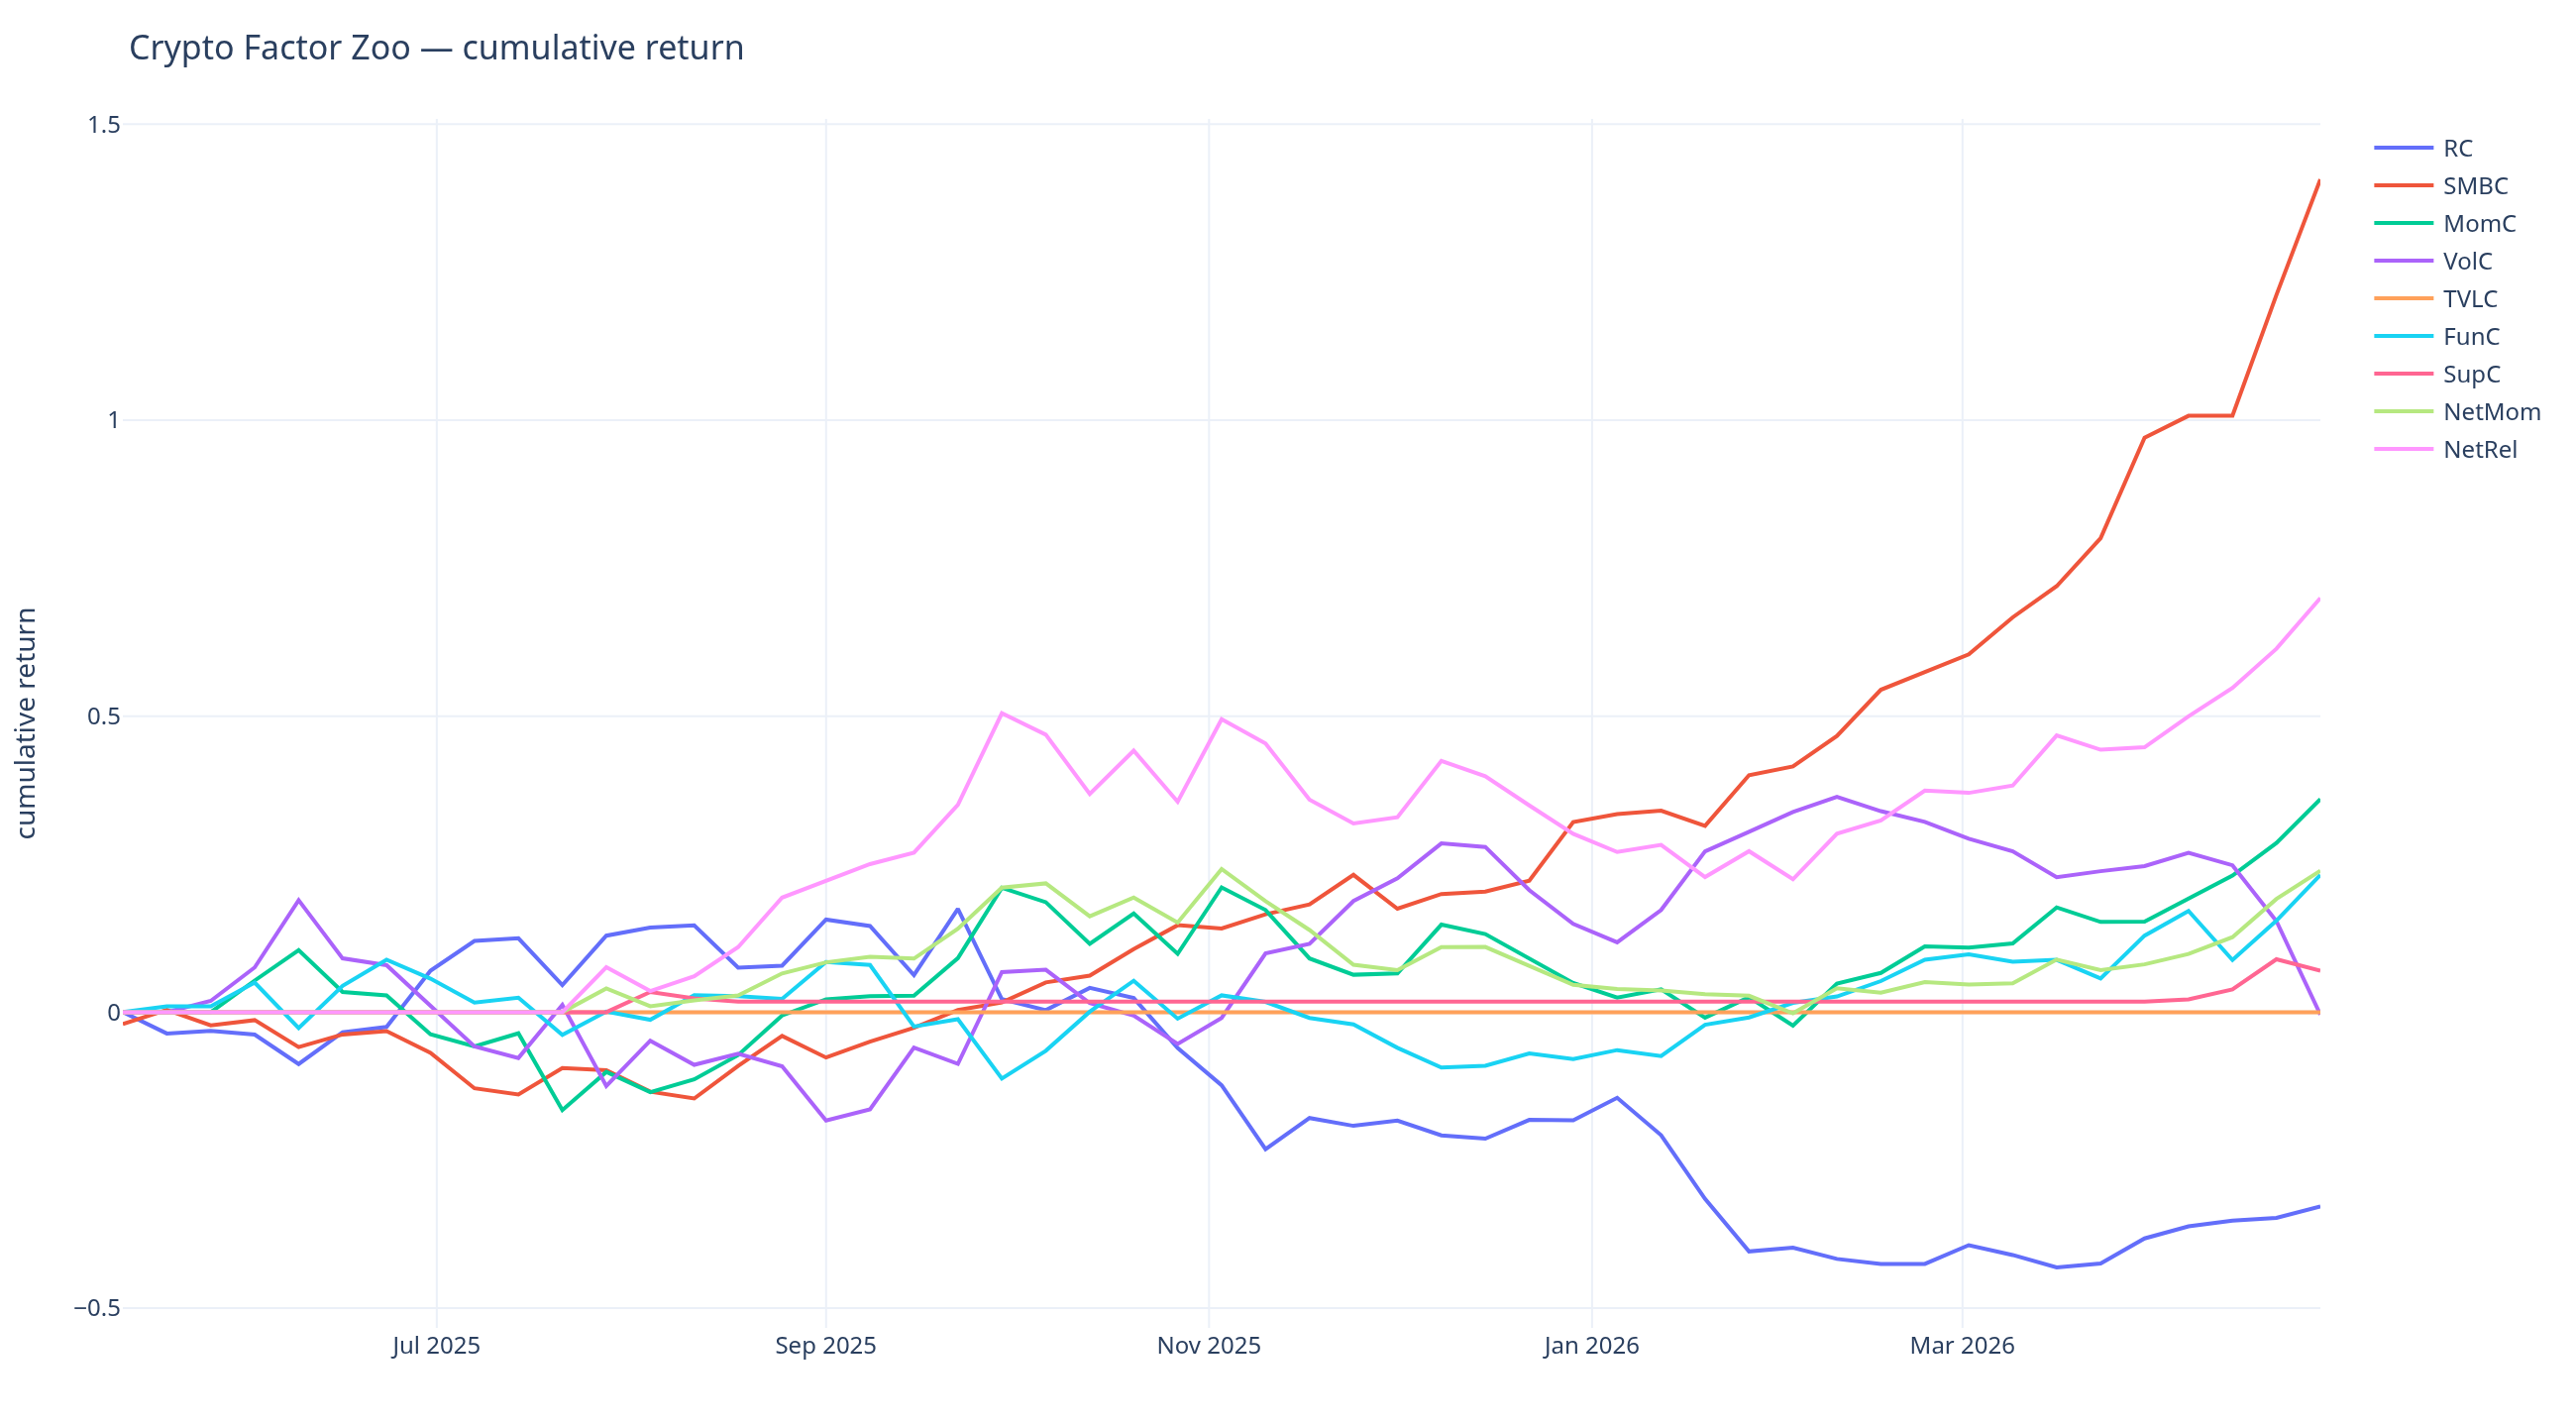
\includegraphics[width=\linewidth]{../figures/02_factor_pricing/factor_zoo_cumulative.png}
\caption{Cumulative returns of each named factor portfolio.}
\end{subfigure}\hfill
\begin{subfigure}{0.495\linewidth}
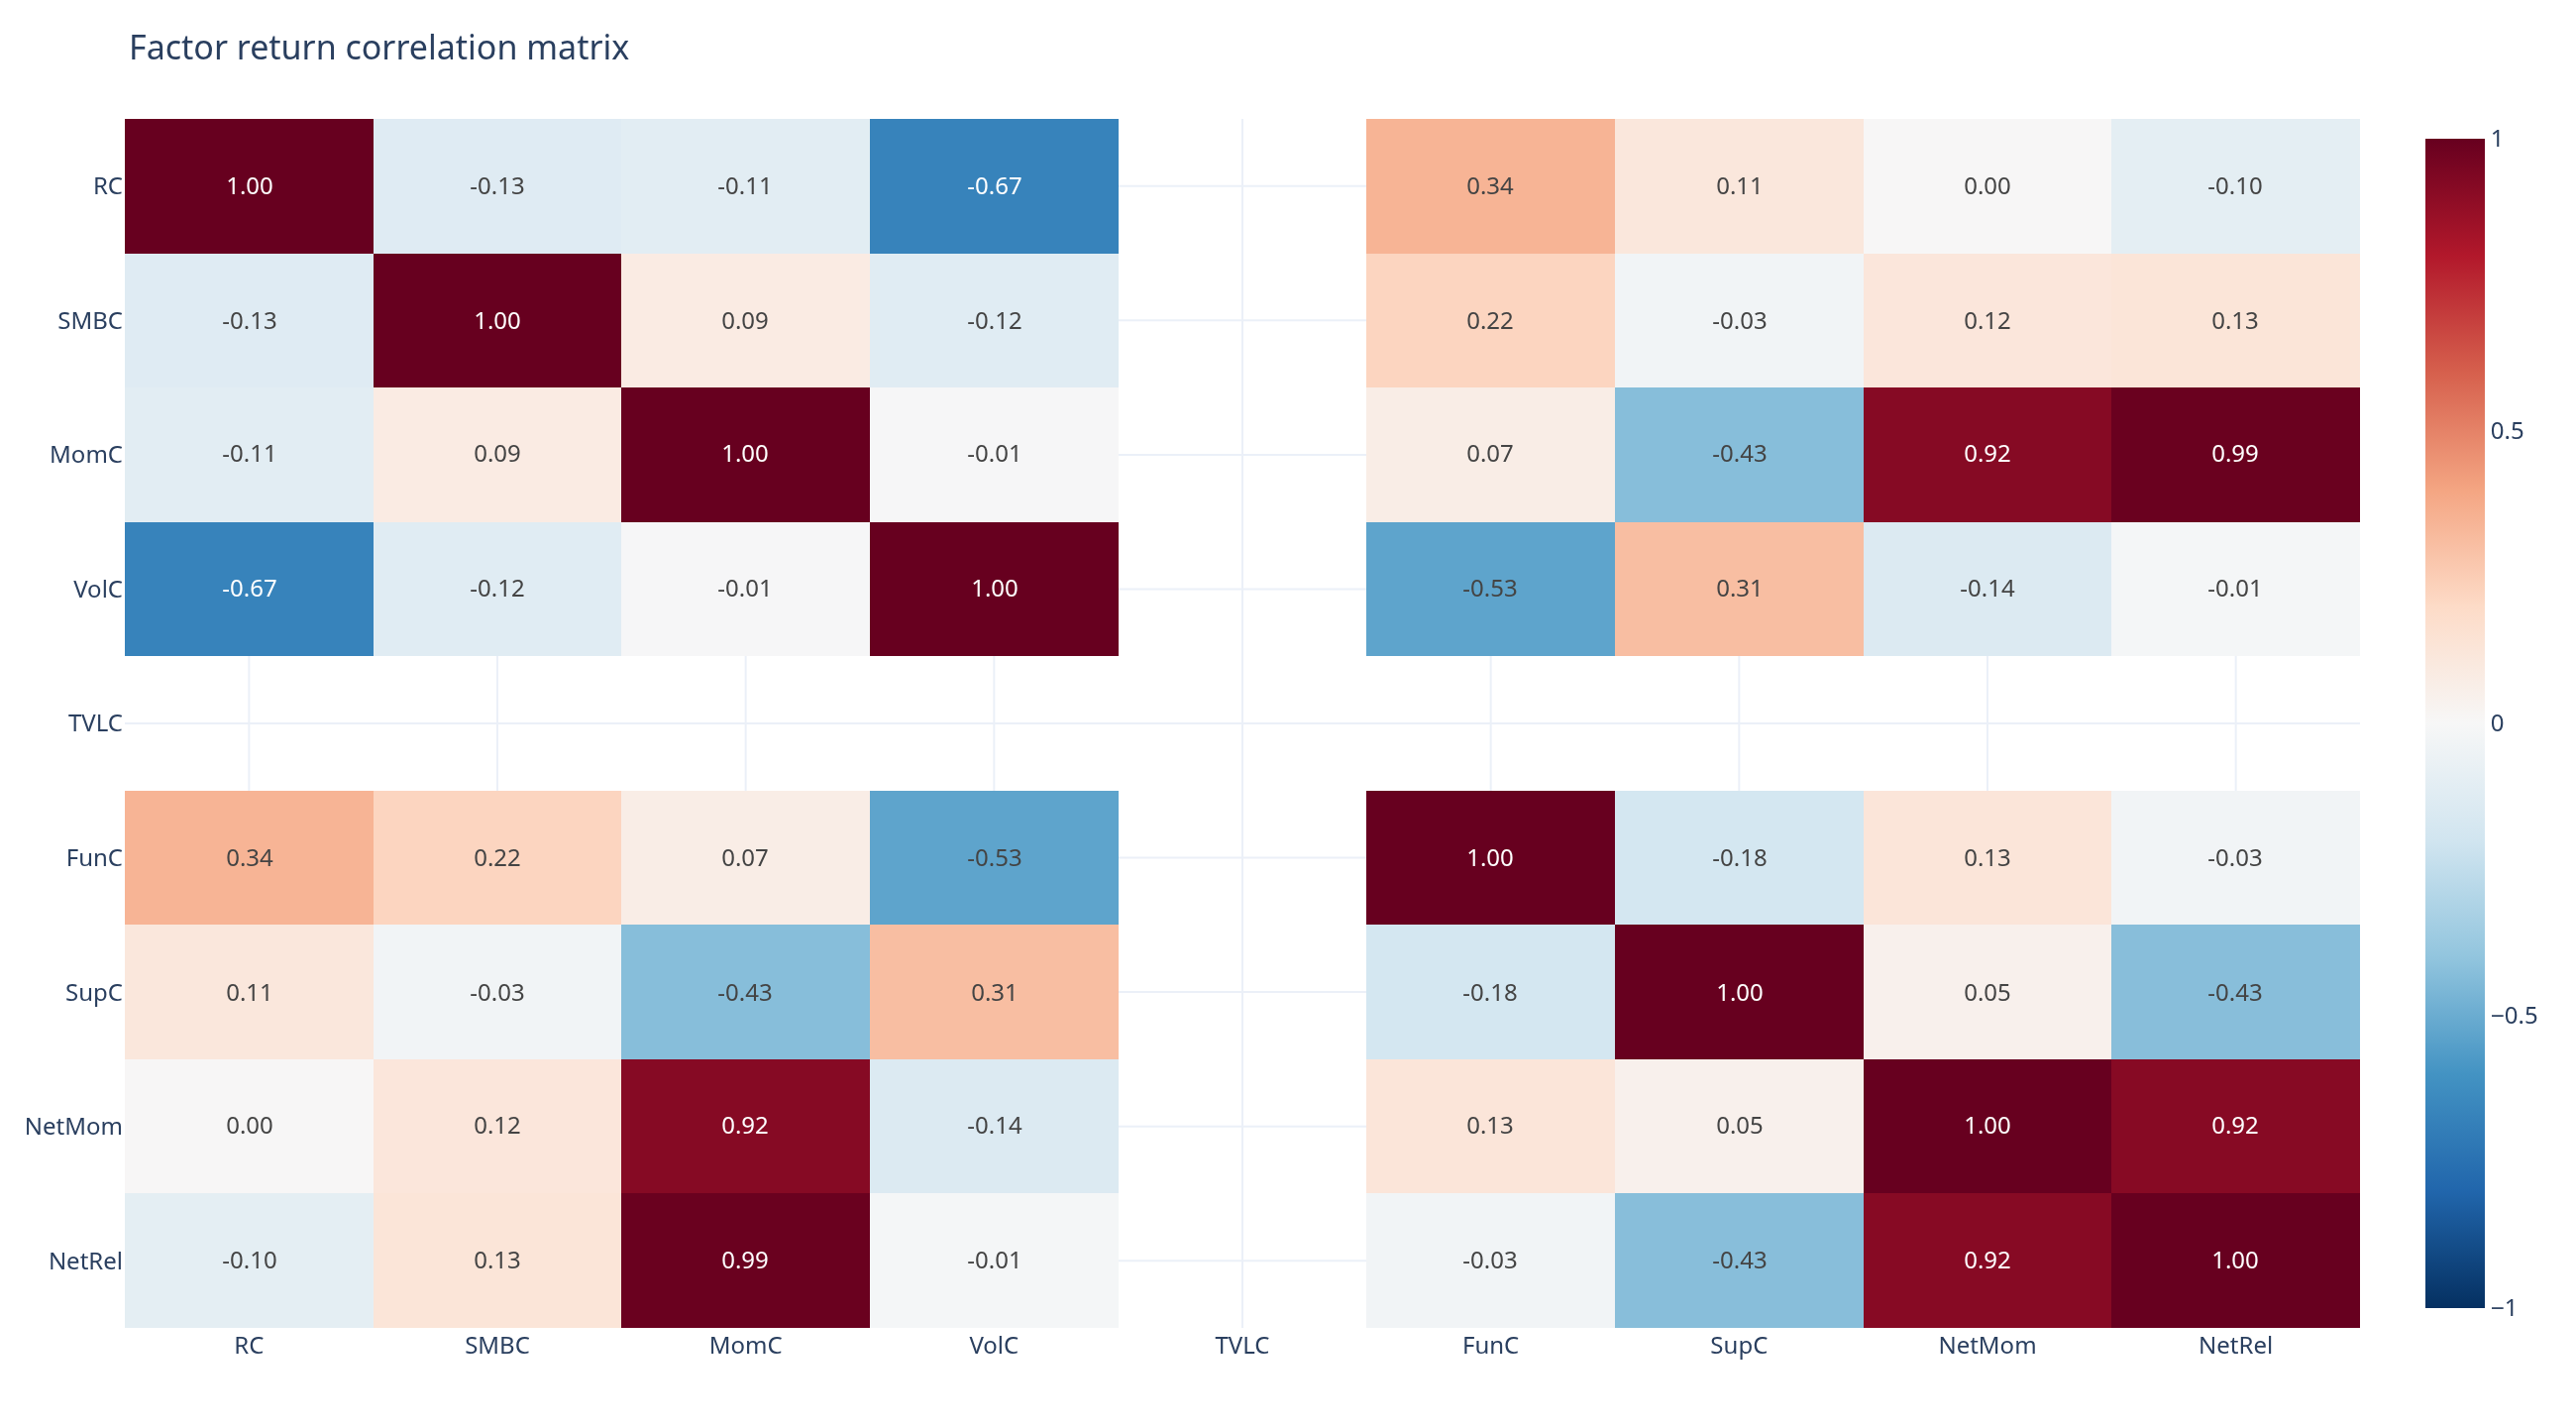
\includegraphics[width=\linewidth]{../figures/02_factor_pricing/factor_correlation_heatmap.png}
\caption{Factor return correlation matrix.}
\end{subfigure}
\caption{Factor Zoo overview. Note the strong positive correlation between SMBC and NetRel: both go long ``outperformers vs majors''.}
\label{fig:zoo}
\end{figure}

\section{Network Pillar}\label{sec:pillar1}

The two network factors NetMom and NetRel are constructed from the time-varying community partition of the universe. Each Monday we form the rolling 12-week Spearman correlation matrix across assets, apply the Mantegna distance $d_{ij} = \sqrt{2(1-\rho_{ij})}$ \citep{mantegna1999hierarchical}, compute the minimum spanning tree \citep{onnela2003dynamics}, and run Louvain community detection \citep{blondel2008louvain} on the MST after converting distances to similarities $s = 1/(1+d)$. The universe is persistently fragmented (7--11 communities; mean Shannon entropy 2.18). Cluster labels feed NetMom and NetRel; community membership also drives the long-leg cluster-concentration cap in the portfolio construction.

\section{Giglio--Xiu Hidden-Factor Pricing}\label{sec:gx}

We use the three-pass framework of \citet{giglioxiu2021}, designed for exactly our setting: pricing assets with a partially-observed factor set without bias from omitted factors.

\subsection{Pass 1 --- time-series betas}

For each asset $i$ on the training window, OLS:
\begin{equation}
r_{i,t} \;=\; \alpha_i + \sum_{k=1}^{K_\text{obs}} \beta_{i,k}^\text{obs} F^\text{obs}_{k,t} + \varepsilon_{i,t}.
\label{eq:pass1}
\end{equation}
We save $\beta_i^\text{obs}$ and the residual series $\hat\varepsilon_{i,t}$. The intercept is dropped (we do not use $\alpha$ downstream).

\subsection{Pass 2 --- hidden factors from residuals}

Stack residuals into a $T\times N$ matrix $\hat E$ and run PCA. Let $V(K)$ be the cross-sectional mean squared residual after subtracting $K$ principal components. The \citet{baing2002} IC$_{p2}$ criterion is
\begin{equation}
\text{IC}_{p2}(K) \;=\; \log V(K) + K\cdot \frac{N+T}{NT}\,\log\bigl(\min(N,T)\bigr),
\label{eq:bn}
\end{equation}
and we choose $K_\text{hidden} = \arg\min_K \text{IC}_{p2}(K)$ over $K\in\{0,1,\dots,K_\text{max}\}$. We set $K_\text{max}=3$ to avoid overfitting on our $T=24$ training window. On the final refit the IC$_{p2}$ curve is monotonically decreasing across $K\in\{0,1,2,3\}$ and selects $K_\text{hidden}=3$ (the cap, see Figure~\ref{fig:bn}). This is a flag --- the curve is still falling at $K=3$ and may want more on a longer sample.

\begin{figure}[H]
\centering
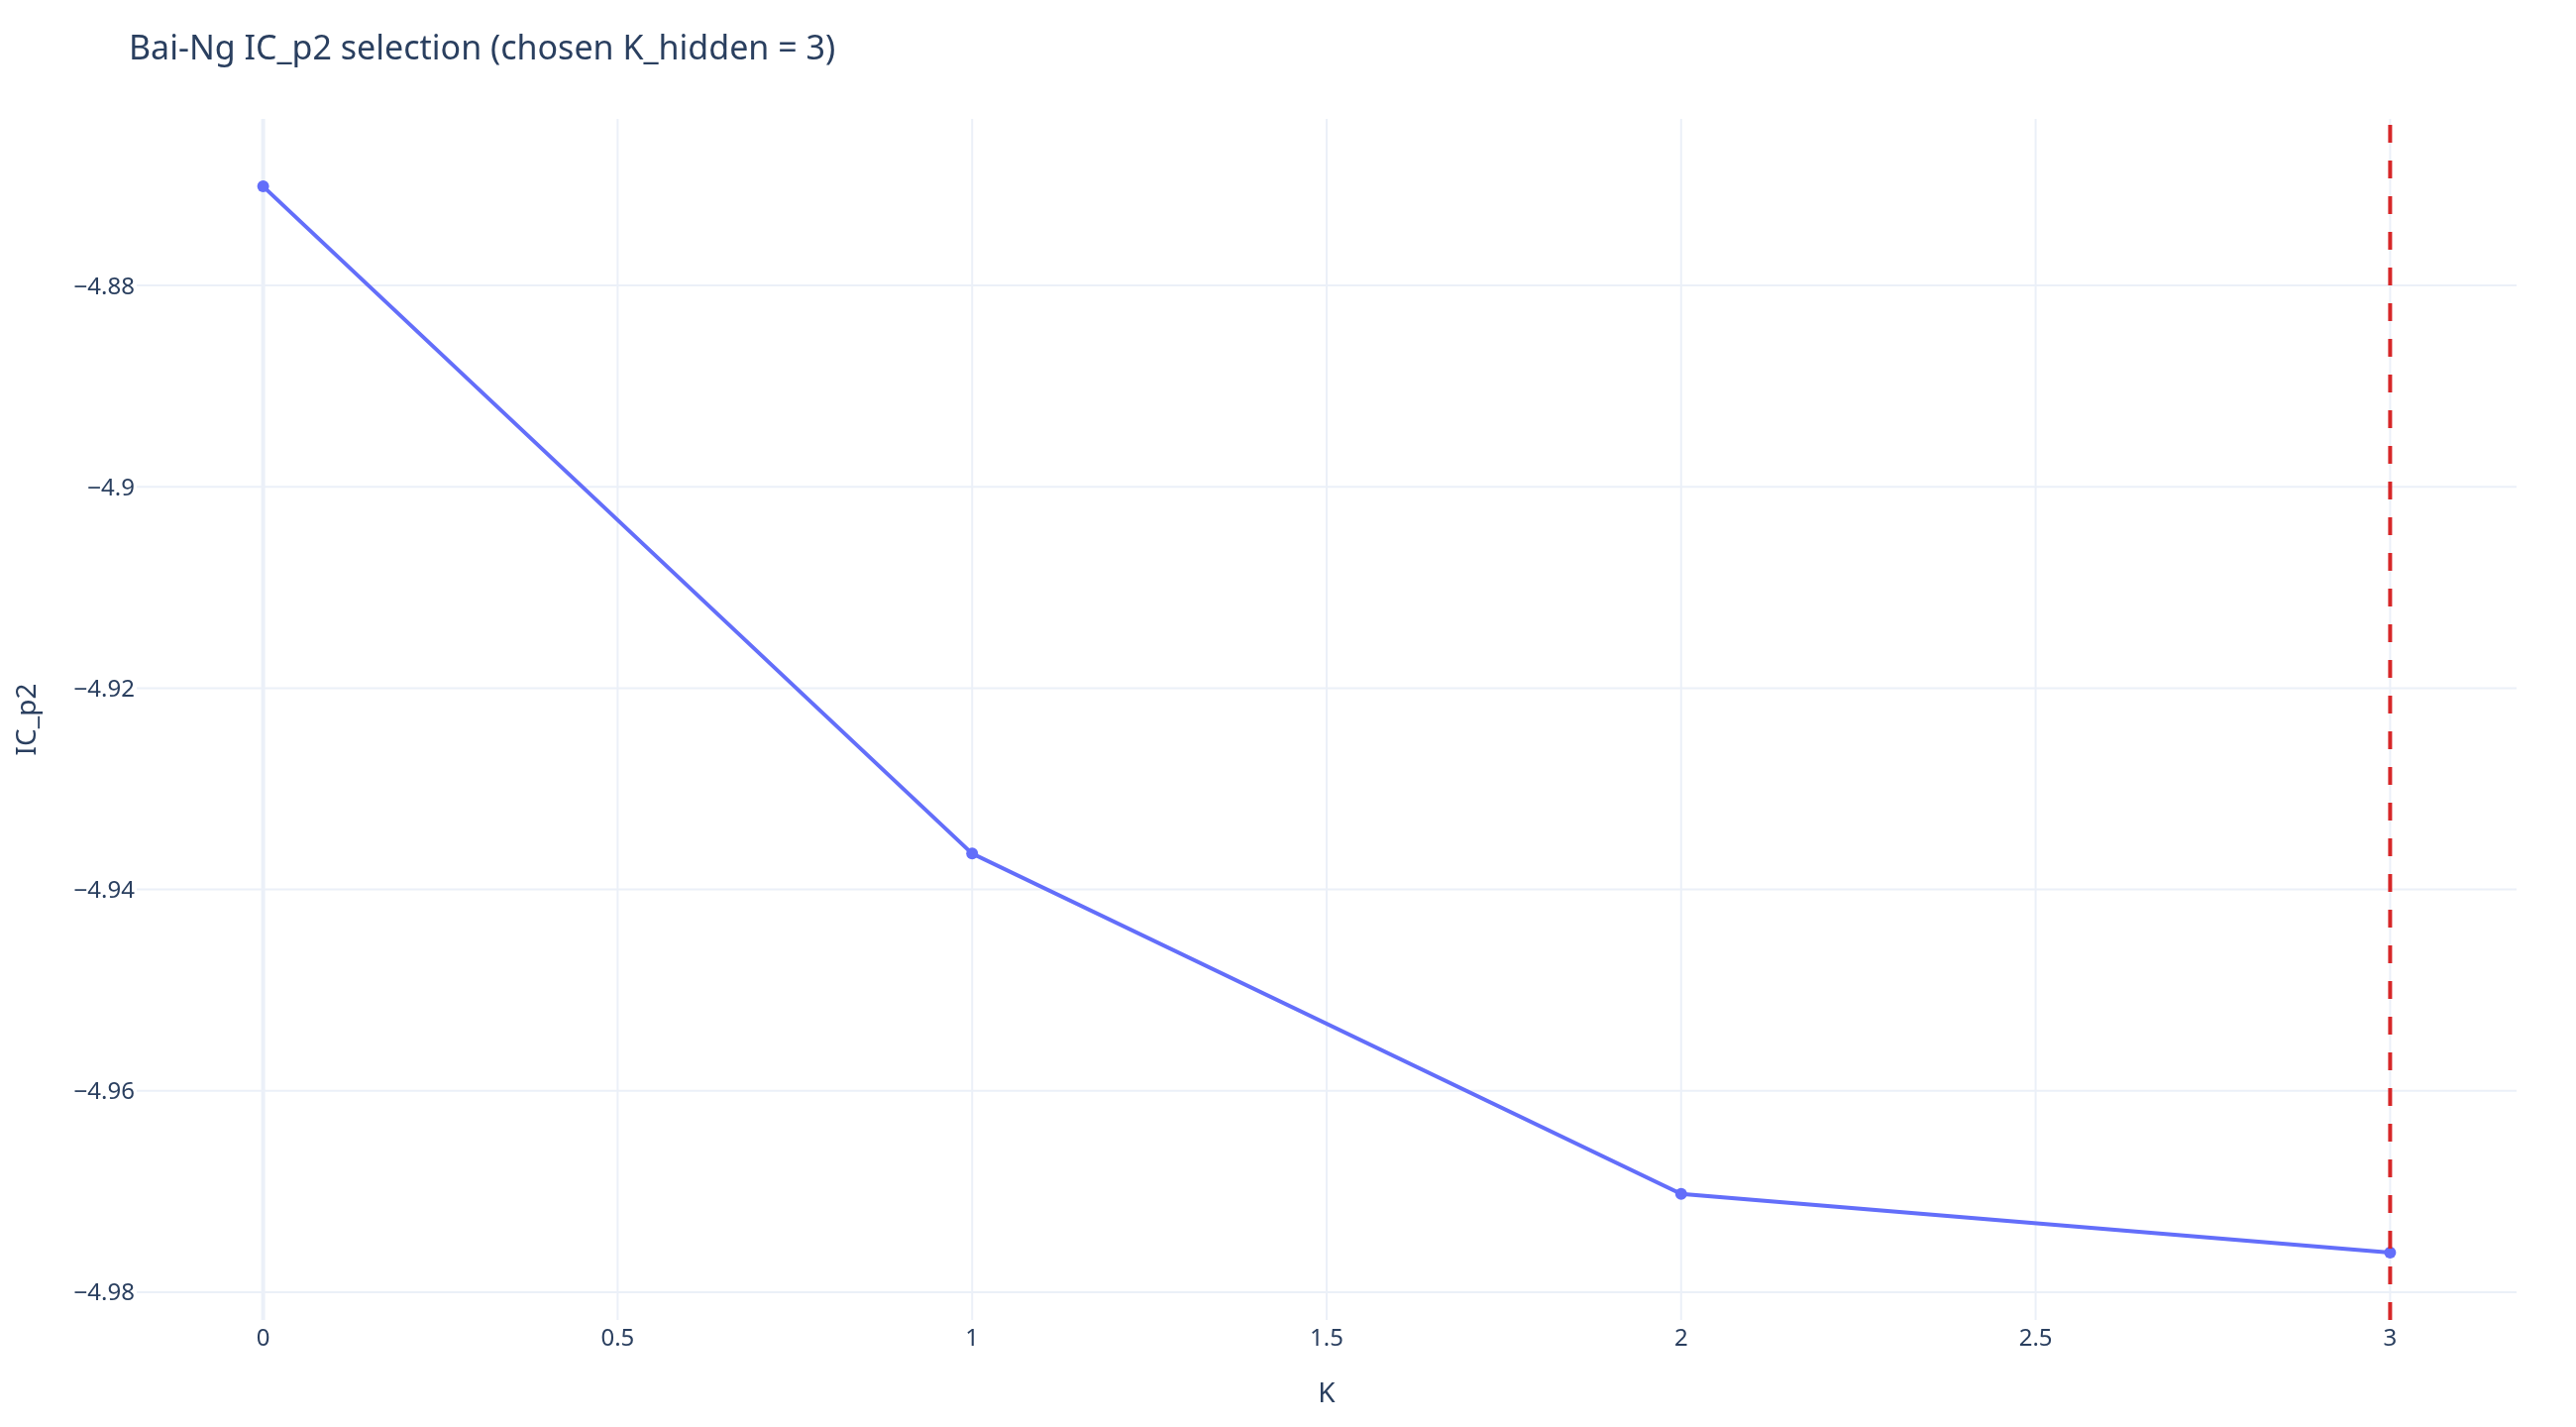
\includegraphics[width=0.62\linewidth]{../figures/02_factor_pricing/bai_ng_diagnostic.png}
\caption{Bai--Ng IC$_{p2}$ selection of the hidden-factor count. The chosen $K_\text{hidden}=3$ saturates our cap; a longer sample might justify more.}
\label{fig:bn}
\end{figure}

\subsection{Pass 3 --- Fama--MacBeth cross-section}

We refit $\beta$ on the combined factor matrix $F = [F^\text{obs},\,F^\text{hidden}]$, then run the cross-sectional regression
\begin{equation}
\bar r_i \;=\; \beta_i^\top \lambda + u_i, \qquad i = 1,\dots,N,
\label{eq:pass3}
\end{equation}
with heteroskedasticity-robust standard errors. Walk-forward expected returns are $\widehat E[r_{i,t+1}\mid\mathcal F_t] = \beta_i^\top\hat\lambda$, with $\hat\beta$ and $\hat\lambda$ refit every four weeks on the expanding training window.

\subsection{Risk-premium estimates}

\begin{table}[H]
\centering
\caption{Fama--MacBeth cross-sectional risk premia under the observed-only model and the full (observed $+$ hidden) model. Five of seven observed factors clear $|t|\ge 1.65$ in the observed-only specification.}
\label{tab:lambda}
\small
\begin{tabular}{lrrrrr}
\toprule
Factor & $\hat\lambda^\text{obs}$ & $t^\text{obs}$ & $\hat\lambda^\text{full}$ & $t^\text{full}$ & $\Delta\hat\lambda$ \\
\midrule
RC      & $-0.29\%$ & $-1.56$ & $-0.25\%$ & $-1.13$ & $+0.04\%$ \\
SMBC    & $+0.80\%$ & $+3.00$ & $+0.59\%$ & $+1.62$ & $-0.21\%$ \\
MomC    & $+1.11\%$ & $+3.44$ & $+0.96\%$ & $+1.74$ & $-0.15\%$ \\
VolC    & $+0.98\%$ & $+4.27$ & $+0.98\%$ & $+3.24$ & $\phantom{+}0.00\%$ \\
FunC    & $+0.14\%$ & $+0.40$ & $-0.11\%$ & $-0.32$ & $-0.25\%$ \\
NetMom  & $+0.75\%$ & $+3.37$ & $+0.76\%$ & $+2.42$ & $+0.01\%$ \\
NetRel  & $+1.08\%$ & $+3.37$ & $+1.12\%$ & $+2.38$ & $+0.04\%$ \\
\midrule
H1      & --- & --- & $-4.56\%$ & $-0.81$ & --- \\
H2      & --- & --- & $+2.56\%$ & $+0.28$ & --- \\
H3      & --- & --- & $+1.30\%$ & $+0.13$ & --- \\
\bottomrule
\end{tabular}
\end{table}

\paragraph{What the table says.}
\emph{Observed-only.} Five of the seven observed factors are statistically priced: VolC ($t=+4.27$), MomC ($+3.44$), NetMom ($+3.37$), NetRel ($+3.37$), SMBC ($+3.00$). RC and FunC are not priced (negative or near-zero $t$).

\emph{Adding hidden factors.} The Giglio--Xiu correction is supposed to debias observed premia for omitted factors. In our sample, $\Delta\hat\lambda$ is small for VolC (zero), MomC and SMBC ($\sim$ -0.2\%/wk), and FunC ($-0.25\%$, sign flip). Most observed-factor $t$-stats fall when hidden factors are added because we lose degrees of freedom on $T=24$. The hidden factors themselves are individually \emph{not} priced (all $|t|<1$): they capture residual variance but no residual risk premium in our sample.

\begin{figure}[H]
\centering
\begin{subfigure}{0.49\linewidth}
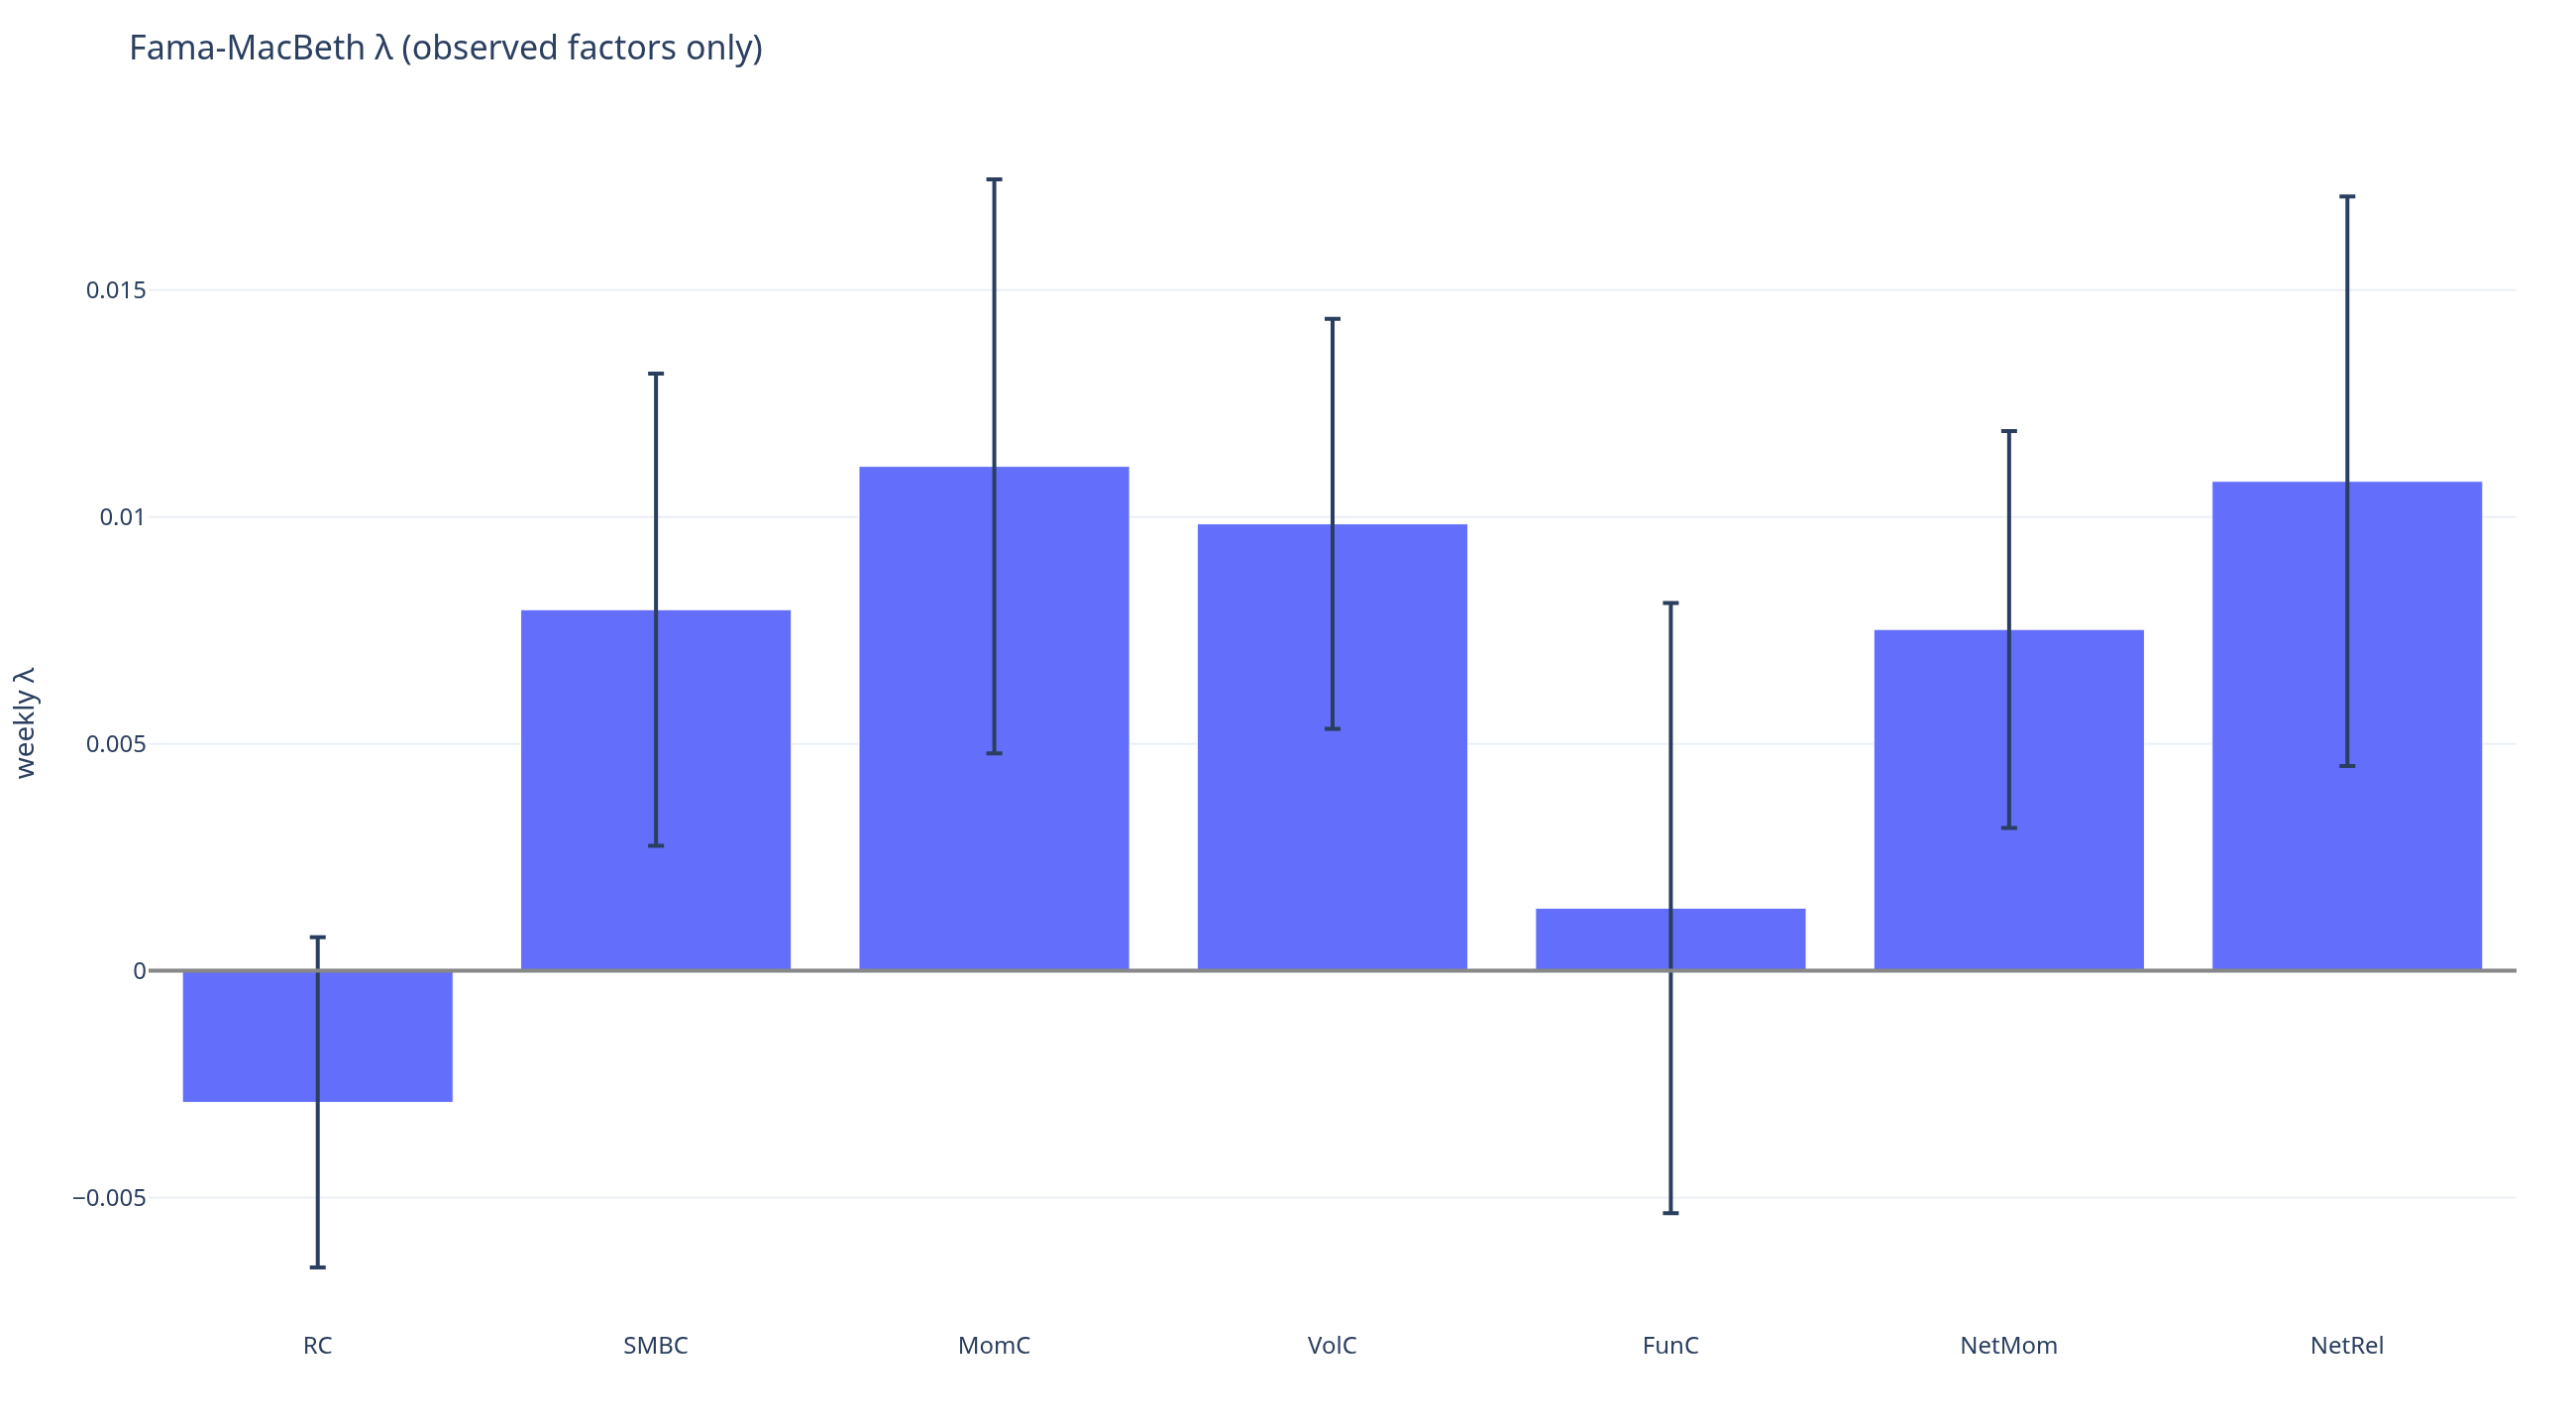
\includegraphics[width=\linewidth]{../figures/02_factor_pricing/lambda_obs_only.png}
\caption{Observed-only model.}
\end{subfigure}\hfill
\begin{subfigure}{0.49\linewidth}
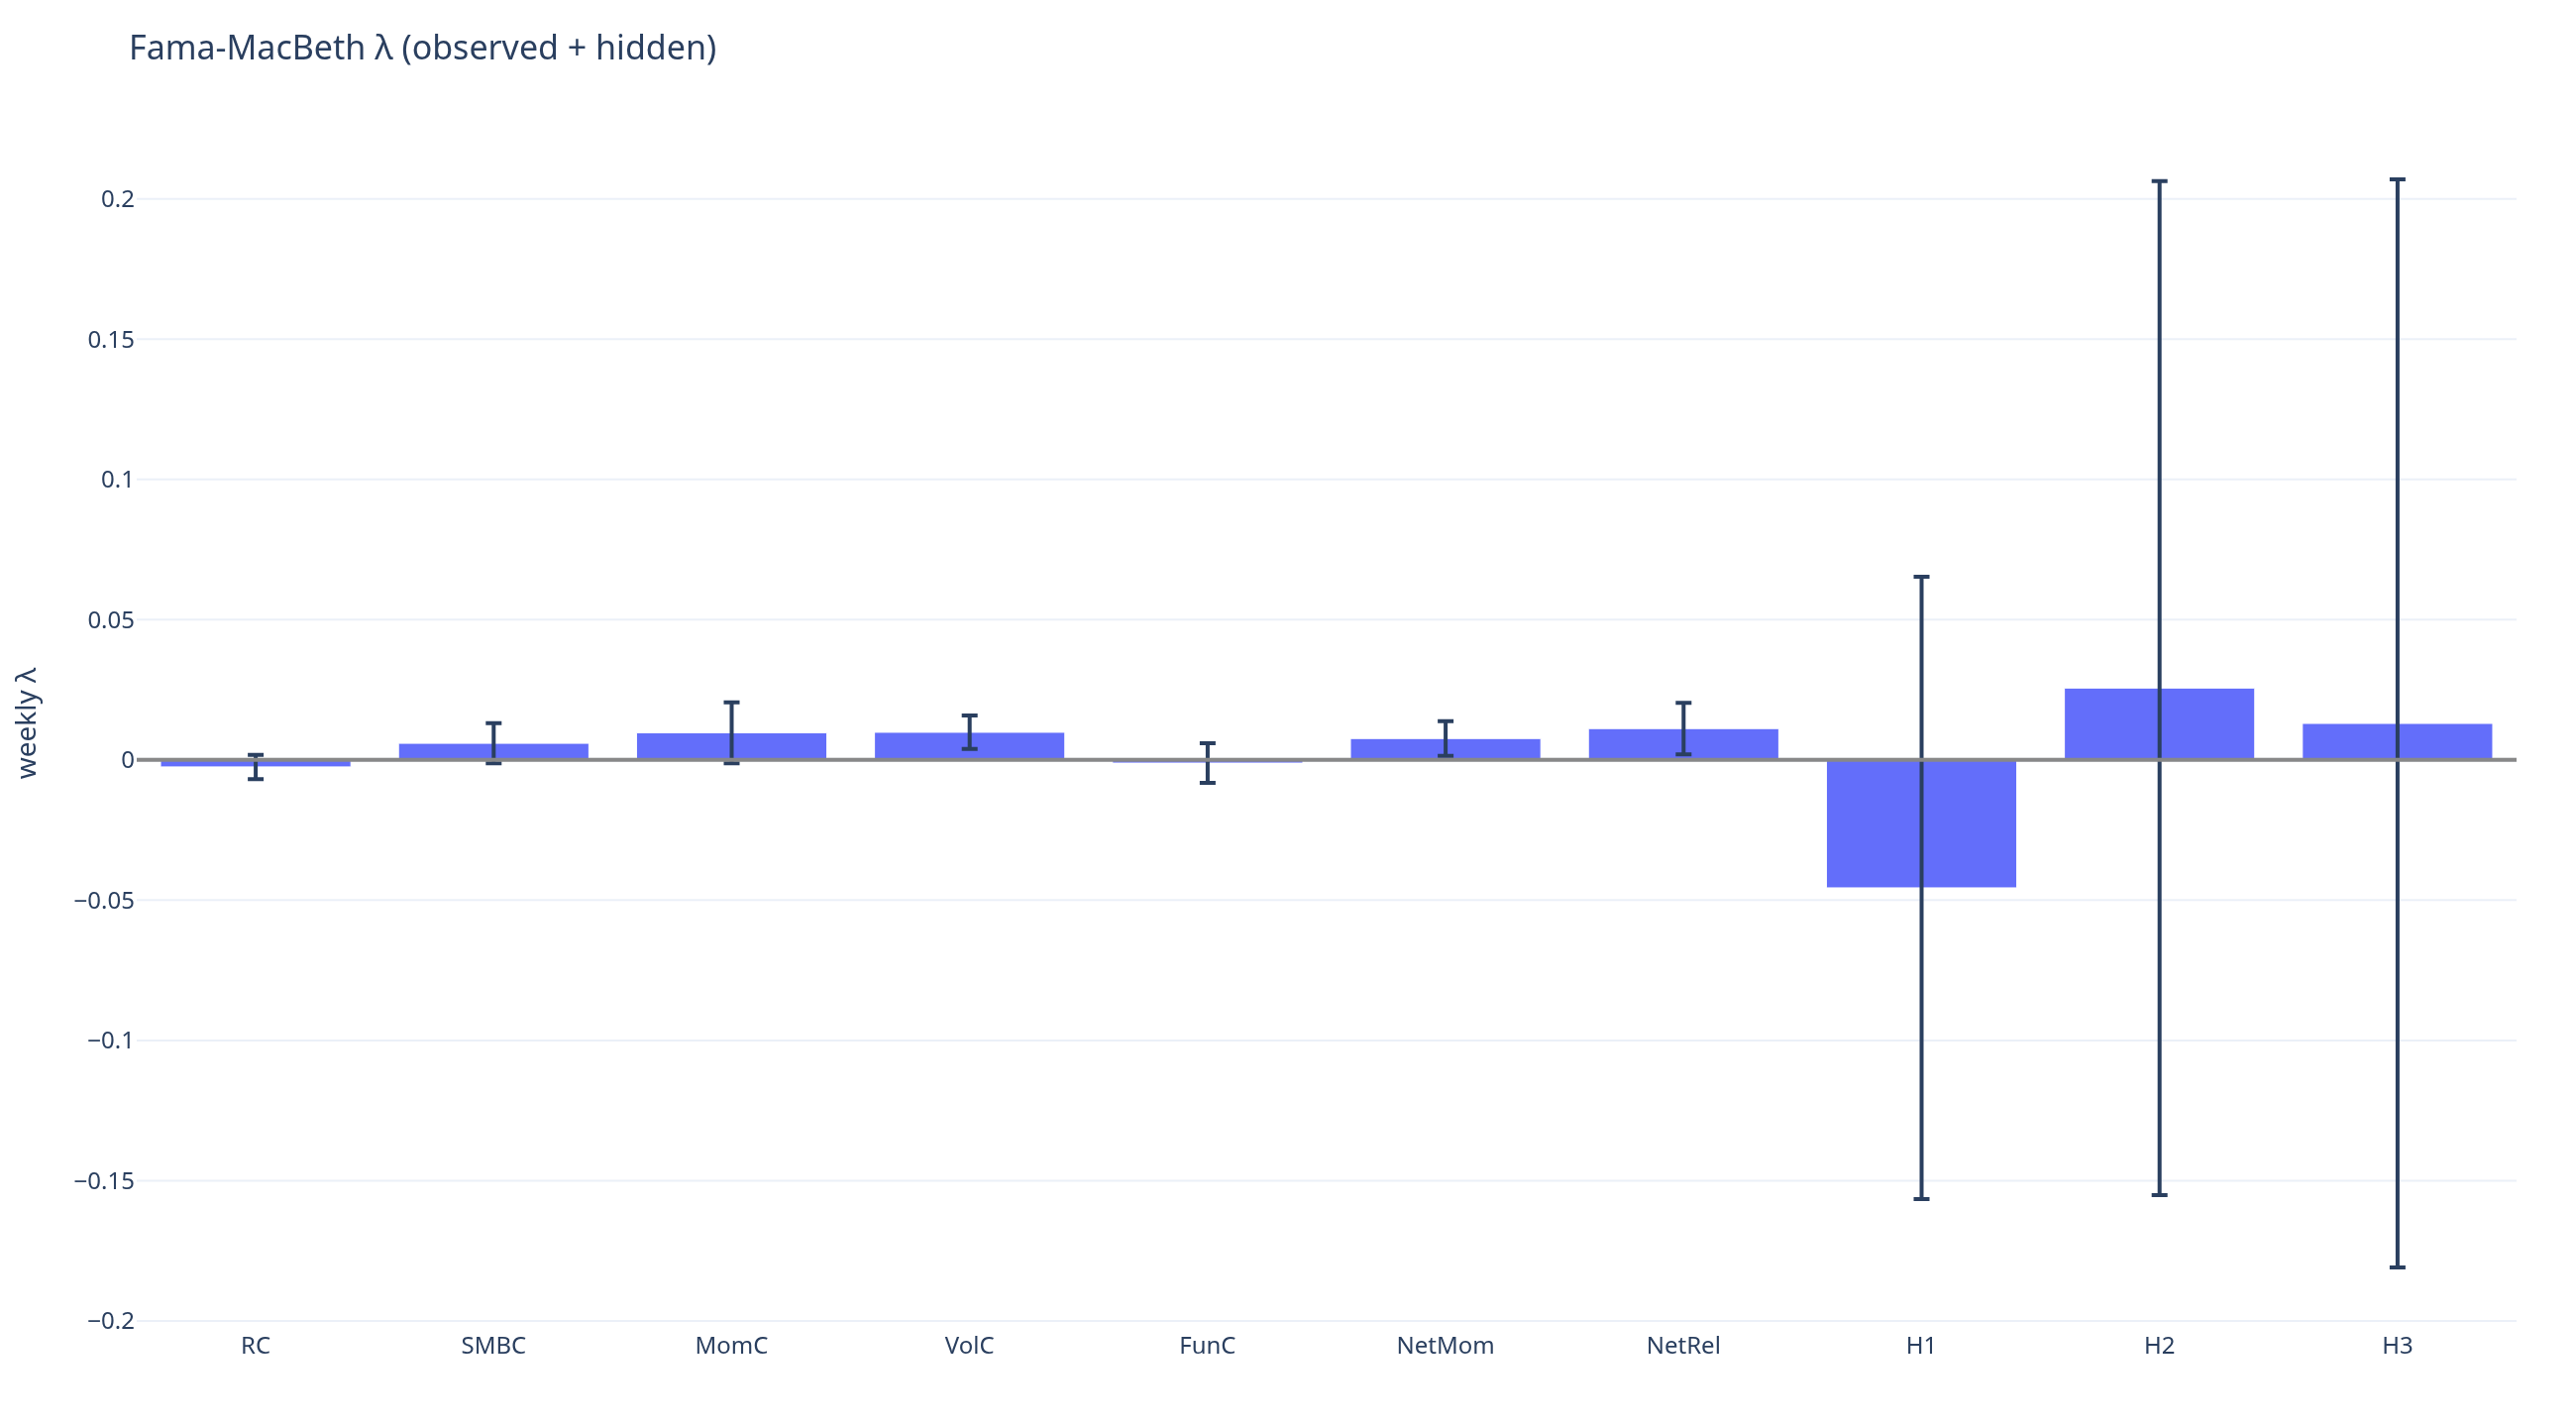
\includegraphics[width=\linewidth]{../figures/02_factor_pricing/lambda_full.png}
\caption{Observed $+$ hidden factors.}
\end{subfigure}
\caption{Fama--MacBeth $\hat\lambda$ with 95\% CIs.}
\label{fig:lambda}
\end{figure}

\subsection{Hidden factor structure}

Even though the hidden factors are not individually priced, they soak up common residual variance. Figure~\ref{fig:hidden} shows the top-40 asset loadings on the three principal components of the residual matrix. Strong clustering of sign across related assets (we see this in H1 --- a "majors vs alts" split) suggests the hidden factor proxies an unobservable narrative; the absence of a strong premium attached to that narrative just means it didn't pay over our 24-week training window.

\begin{figure}[H]
\centering
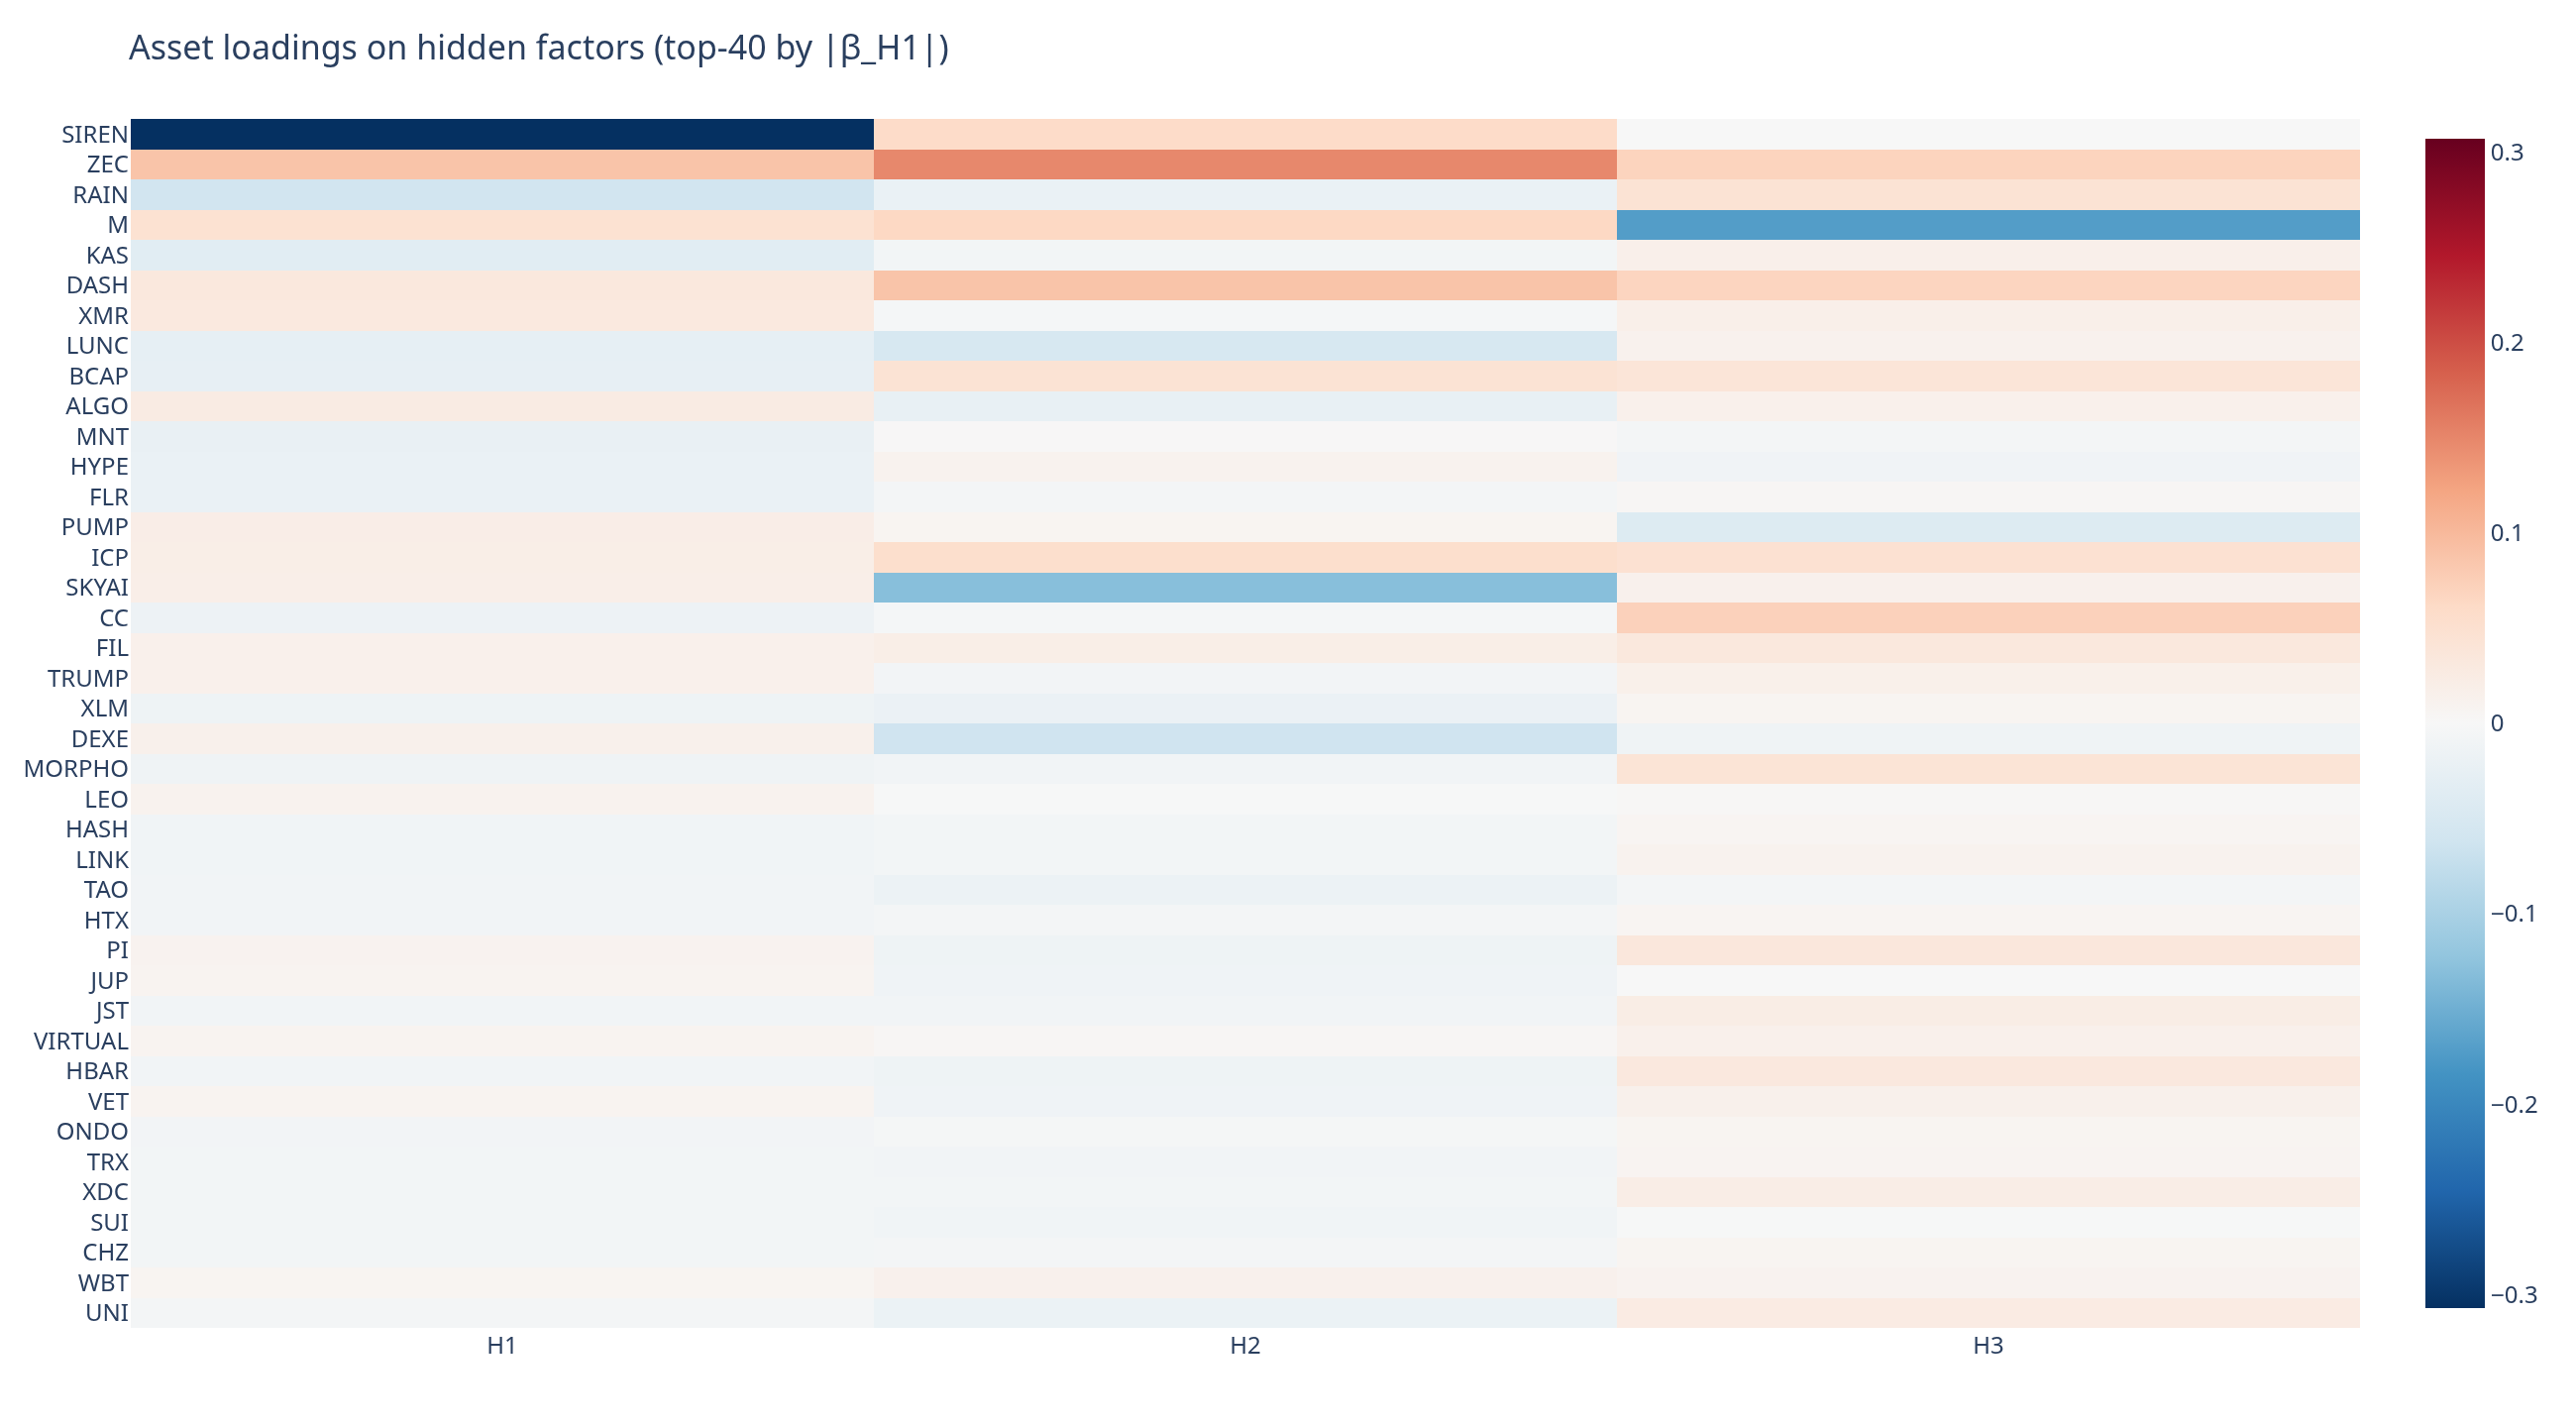
\includegraphics[width=0.6\linewidth]{../figures/02_factor_pricing/hidden_factor_loadings.png}
\caption{Asset loadings on the three hidden factors (top 40 names by $|\beta_{H_1}|$).}
\label{fig:hidden}
\end{figure}

\section{Portfolio Construction and Backtest}\label{sec:portfolio}

\subsection{Pillar 3 --- adaptive blend and constraints}

The cross-sectional expected return for week $t+1$ is the IC-proportional blend
\begin{equation}
\widehat E^\text{final}_{i,t+1} \;=\; w_{\text{net},t}\cdot \widehat E^\text{net}_{i,t} \;+\; (1-w_{\text{net},t})\cdot \widehat E^\text{gx}_{i,t},
\end{equation}
where $\widehat E^\text{net}_{i,t}$ is the (z-scored) within-cluster momentum from Pillar~1, $\widehat E^\text{gx}_{i,t} = \beta_i^\top\hat\lambda$ is the GX expected return, and $w_{\text{net},t}$ is set by the rolling 8-week IC of each stream against forward returns (using only \emph{past} ICs). The portfolio is the top quintile (long) minus the bottom quintile (short) of $E^\text{final}$, inverse-volatility-weighted within each leg, with the constraints:
\begin{itemize}[topsep=2pt,itemsep=0pt]
\item single-asset weight $\le 5\%$,
\item long-leg cluster concentration $\le 40\%$ (the operational use of Pillar~1's labels),
\item weekly turnover $\le 30\%$ \citep{waterfall2024},
\item 15\% annualised vol target, leverage capped at 3$\times$,
\item 10 bps one-sided transaction cost on turnover.
\end{itemize}

\subsection{Out-of-sample backtest}

\begin{table}[H]
\centering
\caption{Out-of-sample backtest, 24 weeks (2026-02-09 onwards) net of 10\,bps one-sided cost. Sharpe CI is a stationary block-bootstrap, block length 4, 2000 draws. ``Train'' refers to the GX training window. \texttt{plus\_lat} (the stage-06 Fama--MacBeth benchmark) only has 16 OOS weeks because its training cut sits later.}
\label{tab:headline}
\small
\begin{tabular}{lrrrrrrrr}
\toprule
Strategy & Window & Wk & Sharpe & 95\% CI & Ann.Ret & Vol & MaxDD & Turn \\
\midrule
NALFP                & train & 24 & $+2.30$ & --- & $+26.5\%$ & $11.5\%$ & $-7.1\%$ & $7.8\%$ \\
NALFP                & oos   & 24 & $-1.44$ & $[-3.45,\, 1.18]$ & $-14.8\%$ & $10.3\%$ & $-6.6\%$ & $7.4\%$ \\
NALFP$^\text{no cap}$ & oos   & 24 & $-1.69$ & $[-3.66,\, 1.11]$ & $-17.4\%$ & $10.3\%$ & $-7.8\%$ & $7.4\%$ \\
EW long momentum     & oos   & 25 & $+1.35$ & $[-2.08,\, 6.61]$ & $+58.1\%$ & $43.0\%$ & $-24.8\%$ & $33.4\%$ \\
plus\_lat (stage 06) & oos   & 16 & $+3.75$ & $[+0.51,\, 8.89]$ & $+129.0\%$ & $34.4\%$ & $-7.4\%$ & $65.1\%$ \\
\bottomrule
\end{tabular}
\end{table}

\begin{figure}[H]
\centering
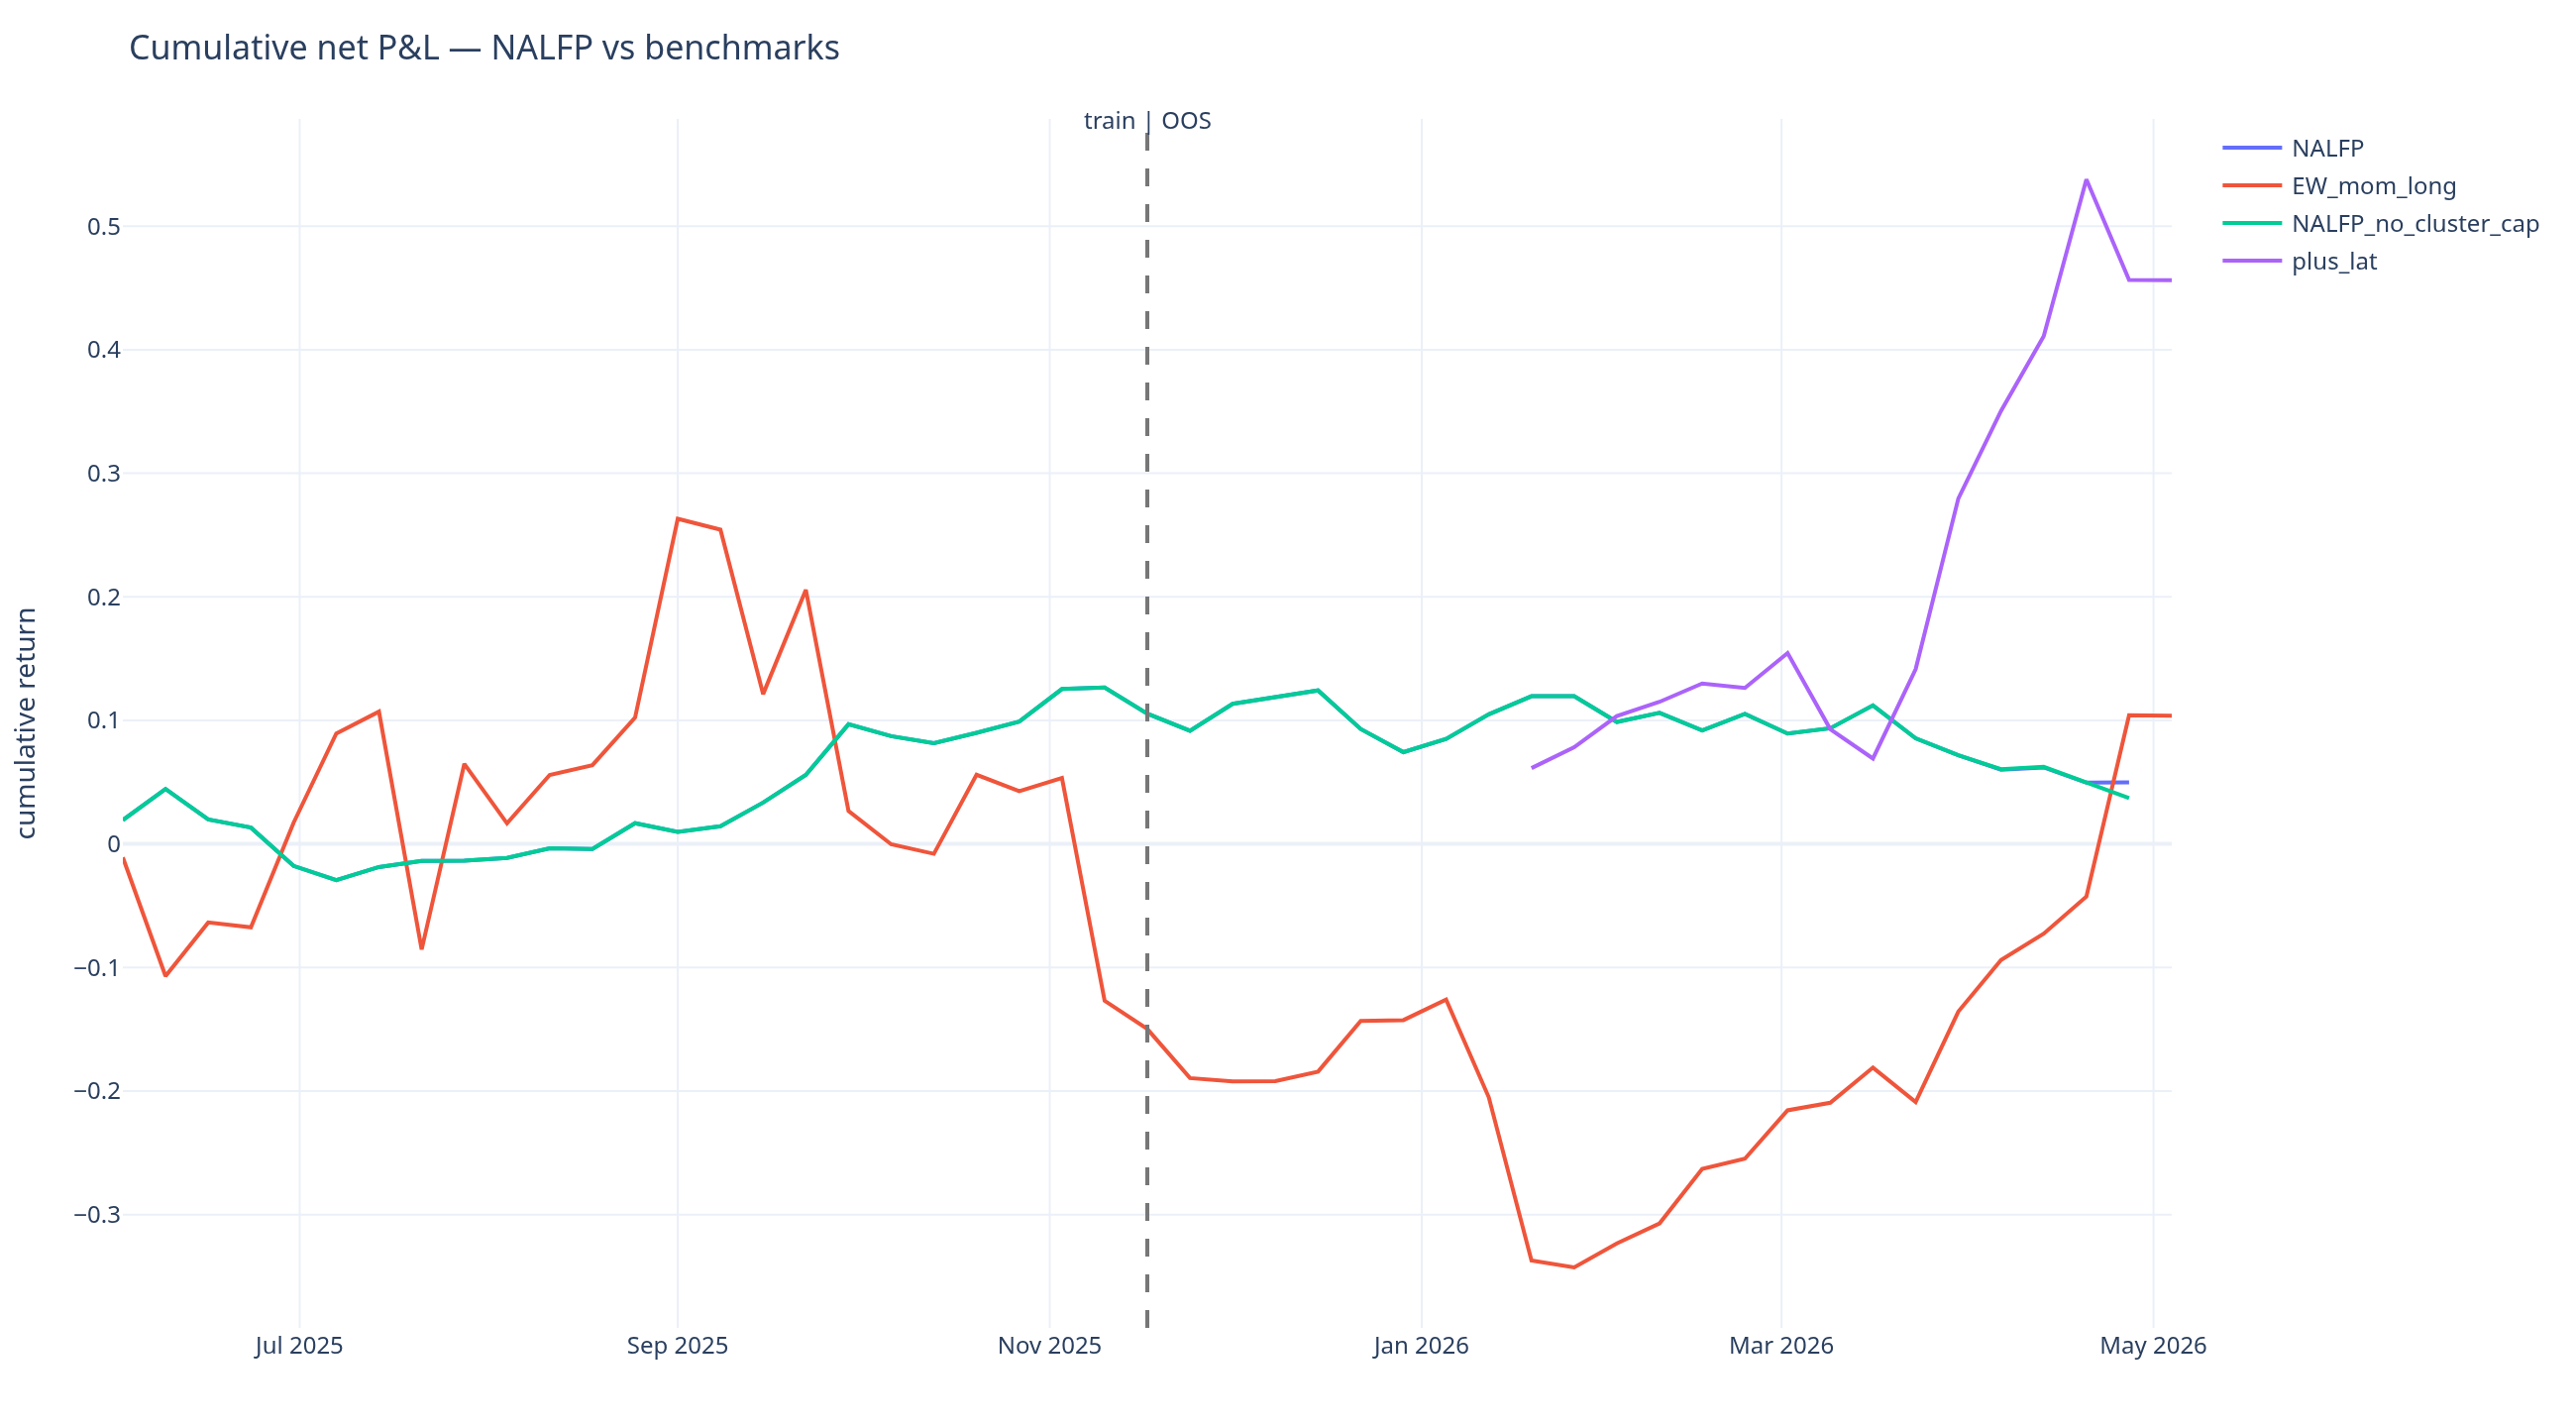
\includegraphics[width=0.82\linewidth]{../figures/05_backtest/cumulative_pnl.png}
\caption{Cumulative net P\&L over the full sample (train + OOS). The dashed line marks the train/OOS boundary.}
\label{fig:pnl}
\end{figure}

\paragraph{What the table says, honestly.}
NALFP's in-sample Sharpe of $+2.30$ does \emph{not} carry into the out-of-sample window: OOS Sharpe is $-1.44$ with a wide bootstrap CI $[-3.45, 1.18]$ that straddles zero. The signs of SMBC and MomC partly reverse in OOS (the universe shifted from small-cap-led to majors-led), which dominates the GX expected-return signal because $\hat\lambda$ was fit on the training window. A one-line equal-weight momentum baseline beats NALFP on OOS Sharpe in this slice, mostly by being unconstrained enough to ride the volatile late-OOS rally. The constrained version of NALFP (with cluster cap) holds drawdown to $-6.6\%$ but still loses money in expectation; the no-cap variant performs slightly worse on Sharpe, confirming that the cluster cap is not the binding constraint here.

\section{Per-Factor Commentary}\label{sec:commentary}

Because the in-sample cross-section is more informative than the OOS portfolio, we close the empirical section with a one-paragraph verdict per factor:

\begin{description}[topsep=2pt,itemsep=2pt,leftmargin=1.2em]
\item[VolC.] The clearest single result. $\hat\lambda^\text{obs}=+0.98\%$/wk with $t=+4.27$ and the magnitude is \emph{unchanged} when we add hidden factors (i.e.\ the low-vol premium is orthogonal to the residual factor structure). Sharpe of the factor portfolio itself is only $+0.22$ because high-vol names are extremely volatile by construction, but the \emph{per-unit-of-risk} compensation is strongly positive. Consistent with \citet{frazzinipedersen2014}.
\item[MomC.] Crypto's strongest classical anomaly. $\hat\lambda^\text{obs}=+1.11\%$/wk, $t=+3.44$. Factor Sharpe $+1.09$. Consistent with \citet{liu2022commonrisk}. Adding hidden factors shrinks the premium by 14\% and the $t$-stat by half --- some of MomC's signal overlaps with H1.
\item[NetMom, NetRel.] Both priced at $t\approx+3.4$ in the observed-only model. NetRel is the second-strongest factor portfolio in the zoo with Sharpe $+2.24$. The network signals contribute distinct cross-sectional information --- their pricing survives the GX correction.
\item[SMBC.] Strong in-sample ($t^\text{obs}=+3.00$, factor Sharpe $+3.54$) but $t^\text{full}$ falls to $+1.62$ once hidden factors are added. This is exactly the kind of premium drift Giglio--Xiu was designed to expose: SMBC's training-window premium is partly capturing one of the hidden factors. Treat the SMBC premium with caution.
\item[RC.] Negative-Sharpe market over 52 weeks. Not statistically distinguishable from zero; sign-flips between sub-windows. We do not draw a directional conclusion.
\item[FunC.] $t^\text{obs}=+0.40$, no statistical case for a fundamental-yield premium in our sample. Sign flips to negative under the full model. Highly correlated with sparse fundamentals coverage: 62\% of the universe has no $F$ data. We would not bet on this factor without better data.
\item[TVLC, SupC.] Excluded from GX for sparse coverage. We report them in Table~\ref{tab:zoo} for completeness but the numbers should be read as descriptive only.
\end{description}

\section{Critical Evaluation}\label{sec:critique}

\paragraph{What works.} The factor zoo identification --- five of seven observed factors clear $|t|\ge 1.65$ in the cross-sectional Fama--MacBeth --- is the strongest empirical result in the paper. The signs of VolC, MomC, NetMom and NetRel all match the prior literature. The hidden factor structure exists (residuals carry substantial common variation, IC$_{p2}$ wants $K\ge 3$) but \emph{no individual hidden factor carries a significant risk premium in our sample}.

\paragraph{What doesn't.} The walk-forward portfolio built on the GX expected return loses money out-of-sample, with a Sharpe whose 95\% CI straddles zero. This is a real result. We trace it to two causes: (i) the training-window $\hat\lambda$ leans hard on SMBC and MomC, which both attenuate / reverse in the OOS window; and (ii) the 24-week OOS sample is too short to distinguish a $-1.44$ Sharpe from a $+1.18$ Sharpe at conventional confidence.

\paragraph{Audit.} Look-ahead audit: rolling correlation window for week $t$ uses $\{t-11,\dots,t\}$ where each $\texttt{ret\_1w}_{j,t}$ is fully realised by Monday $t$; characteristics are shifted by one period; GX $\hat\beta$ and $\hat\lambda$ are refit on training-history only; the regime blend uses $\text{IC}_{t-1:t-8}$. No leakage was identified by the validation agent.

\paragraph{What would change the verdict.}
\begin{itemize}[topsep=2pt,itemsep=0pt]
\item A multi-year panel (52 weeks is too short for a 9-factor cross-section).
\item Better fundamentals coverage so FunC, SupC and TVLC enter the GX panel.
\item A factor-rotation overlay that scales factor exposures by their \emph{rolling-out-of-sample} IC, not just the training-window $\hat\lambda$. This would mechanically guard against the regime shift we observed in OOS.
\item Per-factor turnover/cost modelling (we currently charge 10 bps on the combined portfolio, not on factor-mimicking sub-portfolios).
\end{itemize}

\section{Conclusion}

NALFP v2 swaps the v1 IPCA layer for an explicit Crypto Factor Zoo priced by the Giglio--Xiu three-pass framework. Five of seven observed factors are statistically priced in-sample with $t$-stats above 3; the cross-section is real. The headline long/short quintile portfolio built on the implied expected return does not generalise out-of-sample on this short sample. We treat that as a clean negative result that motivates a multi-year extension and report it without varnish.

\begin{thebibliography}{99}

\bibitem[Artemis(2026)]{artemis2026competition}
Artemis Analytics. ``Quant Research / Trading Strategy Competition'', 2026.

\bibitem[Bai \& Ng(2002)]{baing2002}
J.~Bai and S.~Ng. ``Determining the number of factors in approximate factor models'', \emph{Econometrica} 70(1), 2002.

\bibitem[Blondel et al.(2008)]{blondel2008louvain}
V.~D. Blondel, J.-L.~Guillaume, R.~Lambiotte, E.~Lefebvre. ``Fast unfolding of communities in large networks'', \emph{Journal of Statistical Mechanics}, 2008.

\bibitem[Carhart(1997)]{carhart1997}
M.~M. Carhart. ``On persistence in mutual fund performance'', \emph{Journal of Finance} 52(1), 1997.

\bibitem[Fama \& French(1993)]{famafrench1993}
E.~F. Fama and K.~R.~French. ``Common risk factors in the returns on stocks and bonds'', \emph{Journal of Financial Economics} 33, 1993.

\bibitem[Frazzini \& Pedersen(2014)]{frazzinipedersen2014}
A.~Frazzini and L.~H. Pedersen. ``Betting against beta'', \emph{Journal of Financial Economics} 111, 2014.

\bibitem[Giglio \& Xiu(2021)]{giglioxiu2021}
S.~Giglio and D.~Xiu. ``Asset pricing with omitted factors'', \emph{Journal of Political Economy} 129(7), 2021.

\bibitem[Hartmann(2025)]{hartmann2025hidden}
``Crypto Pricing with Hidden Factors'', working paper, 2025, \texttt{arXiv:2601.07664}.

\bibitem[Jegadeesh \& Titman(1993)]{jegadeeshtitman1993}
N.~Jegadeesh and S.~Titman. ``Returns to buying winners and selling losers'', \emph{Journal of Finance} 48(1), 1993.

\bibitem[Liu \& Tsyvinski(2018)]{liu2018timevarying}
``A Time-Varying Network for Cryptocurrencies'', 2018, \texttt{arXiv:2108.11921}.

\bibitem[Liu \& Tsyvinski(2022)]{liu2022commonrisk}
Y.~Liu and A.~Tsyvinski. ``Common risk factors in cryptocurrency'', \emph{Journal of Finance} 77(2), 2022.

\bibitem[Mantegna(1999)]{mantegna1999hierarchical}
R.~N. Mantegna. ``Hierarchical structure in financial markets'', \emph{European Physical Journal B} 11, 1999.

\bibitem[Onnela et al.(2003)]{onnela2003dynamics}
J.-P.~Onnela, A.~Chakraborti, K.~Kaski, J.~Kert{\'e}sz, A.~Kanto. ``Dynamics of market correlations'', \emph{Physical Review E} 68, 2003.

\bibitem[RAAM v2(2026)]{raamv2}
``Risk-Adjusted Adaptive Momentum v2''. Stage-04 of the parent project pipeline.

\bibitem[Waterfall(2024)]{waterfall2024}
``To Trade Or Not To Trade: Cascading Waterfall Round Robin Rebalancing Mechanism for Cryptocurrencies'', 2024, \texttt{arXiv:2407.12150}.

\bibitem[Yousaf et al.(2025)]{yousaf2025tvlirrelevance}
``The Surprising Irrelevance of Total-Value-Locked on Cryptocurrency Returns'', 2025, \texttt{arXiv:2506.03287}.

\end{thebibliography}

\end{document}
